In the following section we present the results of our implementation and evaluation. We implemented a working prototype for assessing how to integrate LLM-based Automated Bug Fixing into \ac{CI}, and the resulting potentials and limitations of using this system in software development workflows.

The setup and usage of the prototype in a GitHub repository is demonstrated in the first part of this chapter by showcasing the resulting workflow in the GitHub Web \ac{UI}.
In the second part of this section, we present the quantitative evaluation results of applying the prototype to the prepared repository containing the QuixBugs dataset.

\section{Showcase of Workflow} \label{section:showcase}

Setting up the APR system in a repository is achieved by adding 2 files to the ``.github'' directory of the repository. The required files are ``.github/workflows/auto-fix.yml'' and ``.github/scripts/filter\_issues.py''. Furthermore, an ``LLM\_API\_KEY'' secret needs to be added to the repository secrets, and GitHub Actions needs to be granted permission to create pull requests. With these in place, the system is ready to operate.\\
An optional configuration file can be added to the root of the repository. This `.bugfix.yml'' file can be used to override the \ac{LLM} used, max attempts, and naming conventions for labels and branches.

With the system in place and a custom configuration file set up, the APR system is ready to be used in the repository. Bugs can be automatically fixed in two different ways.

One option is processing a single issue immediately when it is created and labeled with ``bug\_v01'', as shown in Figure \ref{fig:issue-trigger}. This allows for fast feedback and quick bug fixing at issue creation and triage\footnote{Issue triage is the process of categorizing and prioritizing issues such as bug reports. \cite{IssuesTriaging}}.

\begin{figure}[H]
    \centering
    \includegraphics[width=1\textwidth]{images/workflow/label_issue.png}
    \caption{Trigger automatic fixing for single issue, Source: screenshot}
    \label{fig:issue-trigger}
\end{figure}

The second way fetches and processes all issues labeled with the ``bug\_v01'' label. Scheduling the workflow at a specific time or dispatching it manually (see Figure \ref{fig:dispatch}) will result in such a run. This offers a more controlled approach to bug fixing, where issues are processed in batches.

\begin{figure}[H]
    \centering
    \includegraphics[width=1\textwidth]{images/workflow/dispatch.png}
    \caption{Manual Dispatch of APR, Source: screenshot}
    \label{fig:dispatch}
\end{figure}

When the workflow is triggered, it creates a new run in the GitHub Actions tab (see Figure \ref{fig:apr-action}). This executes the bug fixing logic described in Section \ref{section:sc}.


\begin{figure}[H]
    \centering
    \includegraphics[width=1\textwidth]{images/workflow/new_run.png}
    \caption{GitHub Action Run, Source: own representation}
    \label{fig:apr-action}
\end{figure}

A run of the APR system can result in two possible outcomes for every processed issue. \\
If a repair attempt is successful, the system creates a pull request containing the proposed code changes and links it to the corresponding issue. This enables users to review the fix and merge it into the main branch. Upon merging, the issue is automatically closed.
Figure \ref{fig:pr} shows an example of a resulting pull request created by the APR system.

\begin{figure}[H]
    \centering
    \includegraphics[width=1\textwidth]{images/workflow/pr.png}
    \caption{Resulting Pull Request, Source: screenshot}
    \label{fig:pr}
\end{figure}

When an issue repair fails after all attempts have been exhausted, the failure is reported to the issue as a comment and the issue is labeled as failed so it won't be picked up again (see Figure \ref{fig:failure-report}). This allows for easy tracking of issues that could not be fixed by the APR system.

\begin{figure}[H]
    \centering
    \includegraphics[width=1\textwidth]{images/workflow/failure_comment.png}
    \caption{Failure Report, Source: screenshot}
    \label{fig:failure-report}
\end{figure}

Issues marked as failed can be picked up again by adding new context to the issue. This can be done by adding a comment to the issue, which will trigger the APR system to pick up the issue again and try to fix it with the added context. This allows for a more dynamic approach to bug fixing, where issues can be fixed as new information becomes available.

%TODO pipeline from comment screenshot

For transparency and debugging, each run provides a live log stream in the GitHub Actions tab (see Figure \ref{fig:log-stream}). This allows users to see the progress of the run and any errors that occur during the execution. For further analysis, logs, metrics, and the complete context objects are published as artifacts for each run, available to download in the run view.
\begin{figure}[H]
    \centering
    \includegraphics[width=1\textwidth]{images/workflow/logs.png}
    \caption{APR log stream, Source: screenshot}
    \label{fig:log-stream}
\end{figure}

Figure \ref{fig:flow} visualizes the resulting workflow of the APR system. The diagram shows the relation between user actions (yellow) and results (blue).

\begin{figure}[H]
    \centering
    \includegraphics[width=0.9\textwidth]{images/flowcharts/flowresult.png}
    \caption{Resulting flow diagram, Source: own representation}
    \label{fig:flow}
\end{figure}

\section{Evaluation Results} \label{section:evaluation-results}

In this section, we present the results of the quantitative evaluation of the implemented APR prototype. The evaluation is based on the collected and calculated data for each run of the prototype. How this data was collected and calculated is described in Section \ref{section:evaluation}. Threats to validity of these results are discussion in Section \ref{section:validity}.

\subsection{Baseline of Evaluation}

The resulting data is based on 24 executions of the APR prototype in the prepared repository (see Section \ref{subsection:environment-setup}), which contains the QuixBugs benchmark. For evaluating the effectiveness, performance, and cost, we ran the APR prototype using twelve selected \acp{LLM} defined in Section \ref{subsection:llm-selection}. All models were tested with one attempt per issue to evaluate zero-shot performance and with a retry loop enabled to compare few-shot performance. This results in 24 pipeline runs each processing 40 issues from the repository.

\subsection{Results}

The following tables and diagrams show the repair success rate, average cost per issue, and average execution time per issue for each model used in the evaluation. Table \ref{table:results} shows the results of the evaluation with one attempt per issue, while the Table \ref{table:retry-results} shows the results with the retry loop enabled and the max attempts set to 3. Diagrams \ref{fig:repair-success-rate}, \ref{fig:avg-cost-per-issue}, and \ref{fig:avg-execution-time-per-issue} visualize and compare the results of the evaluation for each model in a grouped manner. Diagrams \ref{fig:ci-vs-exec-time-per-run-attempts-1} and \ref{fig:ci-vs-exec-time-per-run-attempts-3} show the CI overhead for each model in relation to the execution time of the run. 

\begin{table}[H]
    \centering
    \small
    \caption{Zero shot evaluation results}
    \label{table:results}
    \begin{tabular*}{\textwidth}{@{\extracolsep{\fill}} p{3.5cm} | p{1.3cm} | p{2.5cm} | p{2.7cm} | p{3cm} @{}}
        \hline
        \textbf{Model} & \textbf{ID} & \textbf{Repair Success Rate} & \textbf{Average Cost Per Issue} & \textbf{Average Execution Time Per Issue} \\
        \hline
        \textbf{gemini-2.0-flash-lite}    & G2F-L  & 82.5\% & \$0.0001 & 6.06s \\
        \textbf{gemini-2.0-flash}         & G2F    & 87.5\% & \$0.0002 & 8.18s \\
        \textbf{gemini-2.5-flash-lite}    & G25F-L & 90.0\% & \$0.0002 & 5.07s \\
        \textbf{gemini-2.5-flash}         & G25F   & 92.5\% & \$0.009  & 20.46s \\
        \textbf{gemini-2.5-pro}           & G25P   & 95.0\% & \$0.0713 & 70.09s \\
        \textbf{gpt-4.1-nano}             & GPT4N  & 70.0\% & \$0.0001 & 6.73s \\
        \textbf{gpt-4.1-mini}             & GPT4M  & 90.0\% & \$0.0007 & 8.96s \\
        \textbf{gpt-4.1}                  & GPT4   & 90.0\% & \$0.0033 & 7.42s  \\
        \textbf{o4-mini}                  & O4M    & 90.0\% & \$0.0069 & 23.08s  \\
        \textbf{claude-3-5-haiku}         & C35H   & 0.0\%  & \$0.0024 & 9.17s \\
        \textbf{claude-3-7-sonnet}        & C37S   & 87.5\% & \$0.0069 & 11.72s \\
        \textbf{claude-sonnet-4-0}        & CS40   & 90.0\% & \$0.0103 & 12.96s \\
        \hline
    \end{tabular*}
    \end{table}

    \begin{table}[H]
        \centering
        \small
        \caption{Few shot evaluation results}
        \label{table:retry-results}
        \begin{tabular*}{\textwidth}{@{\extracolsep{\fill}}  p{3.5cm} | p{1.3cm} | p{2.5cm} | p{2.7cm} | p{3cm} @{}}
            \hline
            \textbf{Model} & \textbf{ID} & \textbf{Repair Success Rate} & \textbf{Average Cost Per Issue}  & \textbf{Average Execution Time Per Issue} \\
            \hline
            \textbf{gemini-2.0-flash-lite}    & G2F-L  & 85\%   & \$0.0003  & 13.08s \\
            \textbf{gemini-2.0-flash}         & G2F    & 90.0\% & \$0.0004  & 8.27s \\
            \textbf{gemini-2.5-flash-lite}    & G25F-L & 90.0\% & \$0.0003  & 7.18s \\
            \textbf{gemini-2.5-flash}         & G25F   & 95.0\% & \$0.0111  & 23.65s \\
            \textbf{gemini-2.5-pro}           & G25P   & 97.5\% & \$0.0708 & 68.78s \\
            \textbf{gpt-4.1-nano}             & GPT4N  & 90.0\% & \$0.0003  & 10.61s \\
            \textbf{gpt-4.1-mini}             & GPT4M  & 97.5\% & \$0.0043  & 11.98s \\
            \textbf{gpt-4.1}                  & GPT4   & 97.5\% & \$0.004   & 7.45s \\
            \textbf{o4-mini}                  & O4M    & 100\%  & \$0.007   & 21.54s \\
            \textbf{claude-3-5-haiku}         & C35H   & 15.0\% & \$0.0076  & 23.98s \\
            \textbf{claude-3-7-sonnet}        & C37S   & 95.0\% & \$0.0085  & 27.16s \\
            \textbf{claude-sonnet-4-0}        & CS40   & 92.5\% & \$0.0117  & 16.80s \\
            \hline
        \end{tabular*}
    \end{table}

\begin{figure}[H]
    \centering
    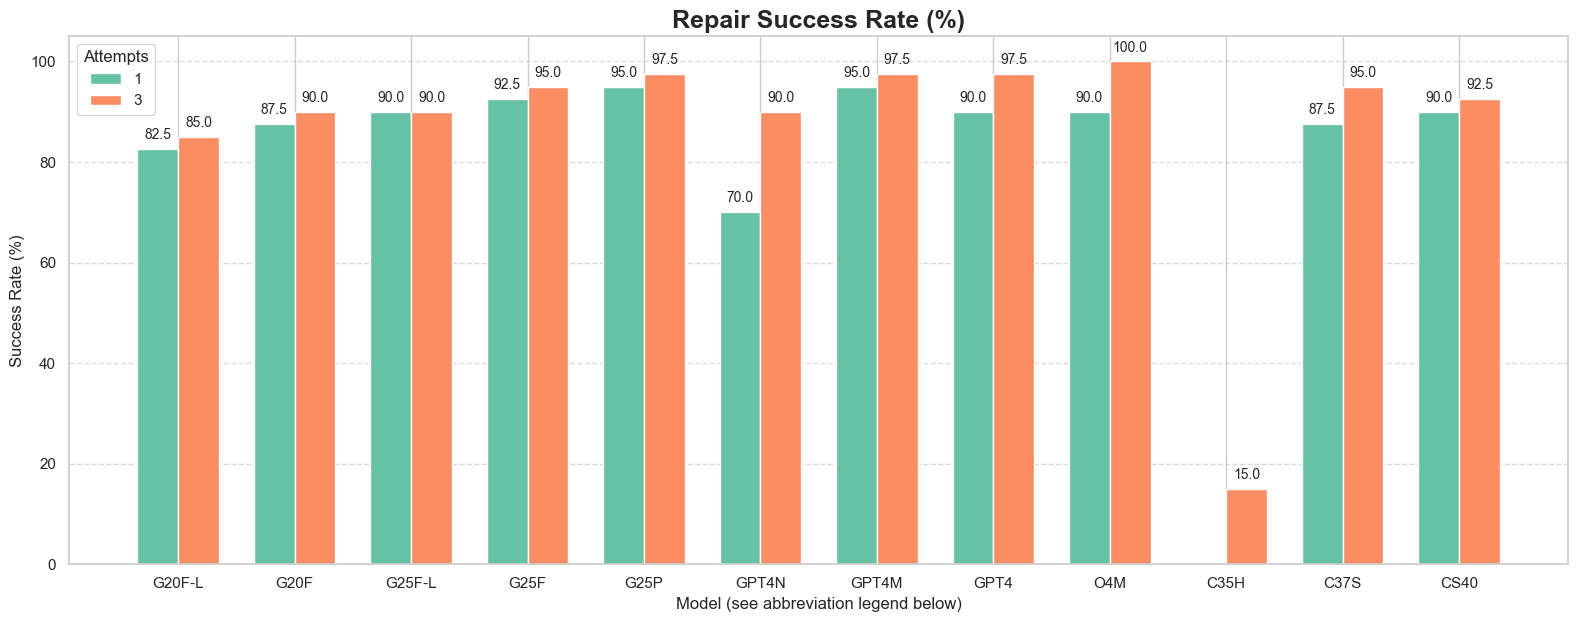
\includegraphics[width=1\textwidth]{images/diagrams/repair_success_rate_per_model_grouped.png}
    \caption{Repair Success Rate per Model, Source: own representation}
    \label{fig:repair-success-rate}
\end{figure}

\begin{figure}[H]
    \centering
    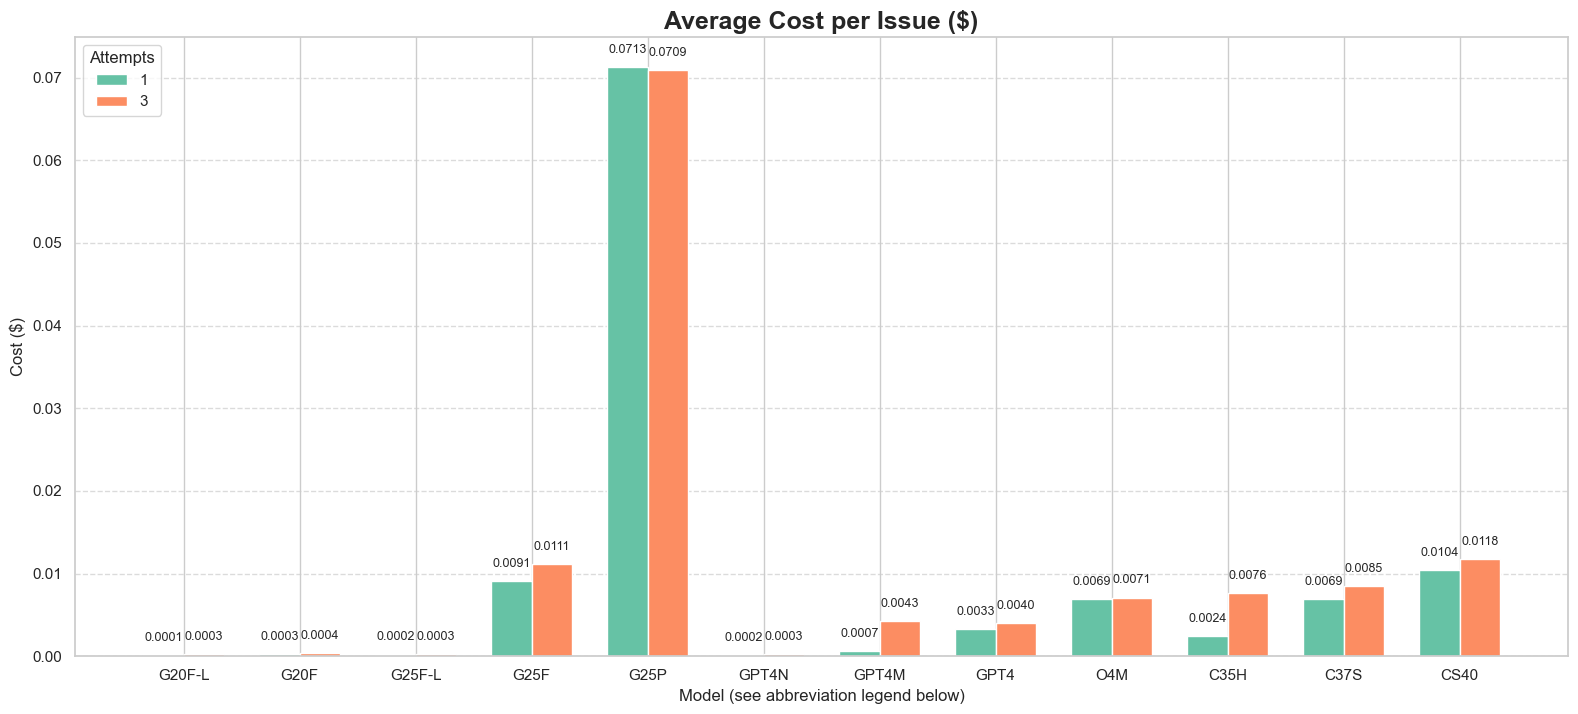
\includegraphics[width=1\textwidth]{images/diagrams/avg_cost_per_issue_per_model_grouped.png}
    \caption{Average Cost per Issue per Model, Source: own representation}
    \label{fig:avg-cost-per-issue}
\end{figure}

\begin{figure}[H]
    \centering
    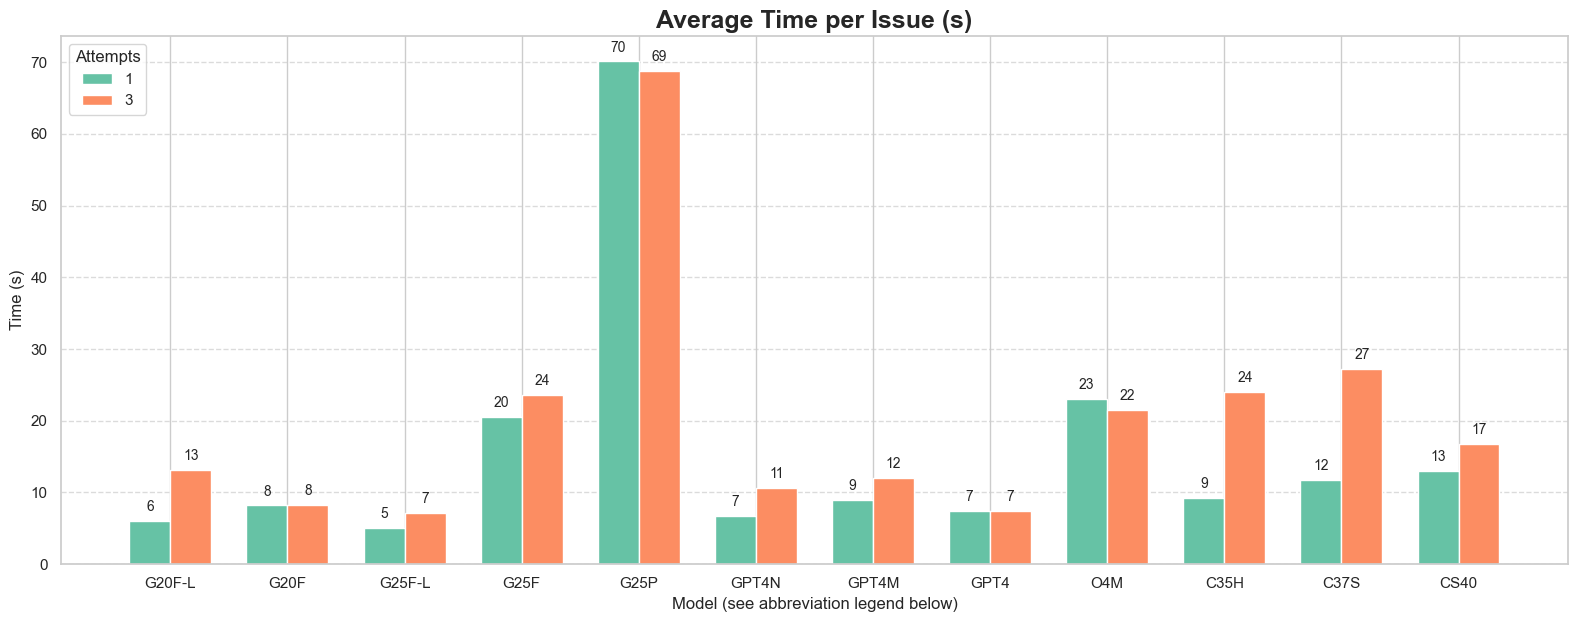
\includegraphics[width=1\textwidth]{images/diagrams/avg_execution_time_per_issue_per_model_grouped.png}
    \caption{Average Execution Time per Issue per Model, Source: own representation}
    \label{fig:avg-execution-time-per-issue}
\end{figure}

\begin{figure}[H]
    \centering
    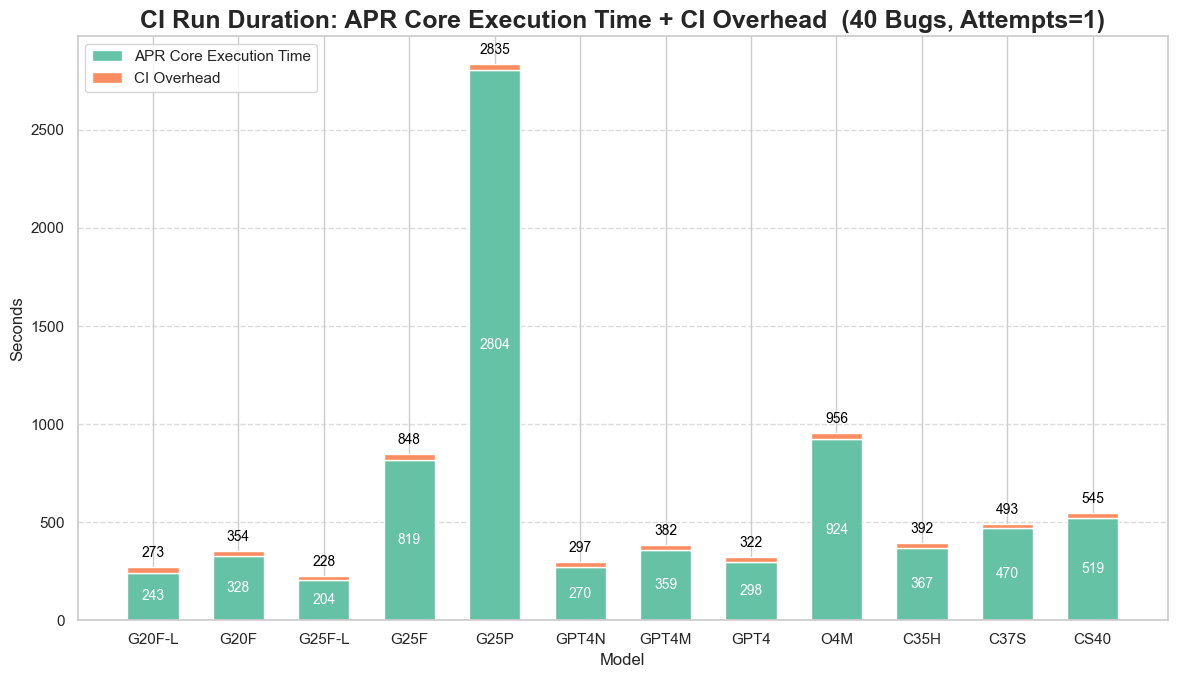
\includegraphics[width=1\textwidth]{images/diagrams/ci_vs_exec_time_per_run_stacked_attempts_1.png}
    \caption{CI Overhead per Run with 1 Attempt, Source: own representation}
    \label{fig:ci-vs-exec-time-per-run-attempts-1}
\end{figure}

\begin{figure}[H]
    \centering
    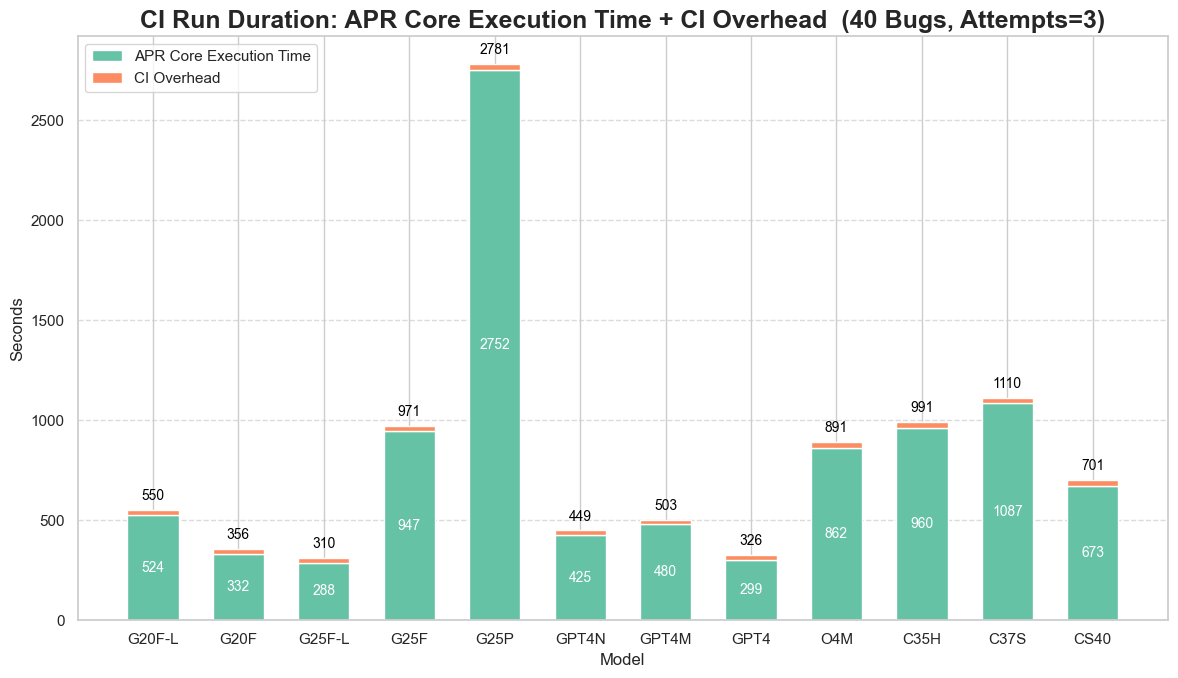
\includegraphics[width=1\textwidth]{images/diagrams/ci_vs_exec_time_per_run_stacked_attempts_3.png}
    \caption{CI Overhead per Run with 3 Attempts, Source: own representation}
    \label{fig:ci-vs-exec-time-per-run-attempts-3}
\end{figure}


The full set of resulting data can be found in the ``apr\_evaluation'' directory of the ``quixbugs-apr'' repository, listed in the Appendix \ref{chapter:appendix}.